\section{Experimental setting and implementation details}
\label{appendix:experimental_settings}
In this section, we detail the protocols and implementation specifics underlying all our evaluations. 
All experiments were run on a single machine equipped with an NVIDIA A100 80 GB GPU under CUDA 12.6 and NVIDIA driver 470.199.02, using PyTorch 2.5.1.

\subsection{Exploratory experiment on spectrum bias}
\label{appendix:exp-spectrum-bias}

To isolate the effect of spectral content on generalization, we generate two synthetic datasets with identical noise level \(\sigma=0.1\) but different frequency composition.

\paragraph{Data generation.} We sample \(N=50{,}000\) inputs for each group; for the low-frequency dataset (Group A) we set \(y = x + \mathcal{N}(0,\sigma^2)\), and for the high-frequency dataset (Group B) we set \(y = x + \frac{\sin(\pi x)}{\pi x} + \mathcal{N}(0,\sigma^2)\). A fixed validation set of 10,000 points is used to track generalization error.

\paragraph{Model and training.}  
Each model is a three-layer MLP (100–100 hidden units, ReLU). We train for 160 steps using Adam (learning rate \(3\times10^{-4}\)) and batch size 1000. After every parameter update, we compute the MSE on the validation set and log the result. The different positions on the x-axis in Figure~\ref{fig:impact} correspond to these intermediate results recorded during the training process.

\subsection{Small-scale validation}  
\label{appendix:small-scale-validation}   
We validate CADS on a reduced‐scale MNIST classification task using a simple convolutional network. All experiments use a fixed training set of 1,000 examples and batch size 1,000. We optimize under an epoch‐based budget of 20 epochs. The selection parameters $\bm{s}\in\mathbb{R}^{|D|}$ are initialized as  
\(
\bm{s} \;=\; v \cdot \bm{1}, 
\quad v \in \{0.2,\,0.4,\,0.6,\,0.8\},
\quad \bm{1}\in\mathbb{R}^{|D|} \text{ is the all-ones vector}.
\)
We solve the bilevel problem with Adam for both the network parameters $\theta$ (learning rate $5\times10^{-3}$) and the selection weights $\bm{s}$ (learning rate $5\times10^{-2}$). The outer loop runs for 300 iterations with variance reduction and gradient clipping enabled.

\paragraph{Network architecture.}  
We employ a simple convolutional model: two convolutional layers with $5\times5$ kernels and channel counts $\{32,64\}$, each followed by ReLU and optional $2\times2$ max‐pooling; the feature map is flattened ($4\times4\times64=1024$ units) and passed through a fully connected layer of 128 units with ReLU; a final linear layer outputs class logits. Input normalization by fixed mean and standard deviation is applied when enabled. No dropout is used.  

\subsection{Heterogeneous data sources: small‐scale experiments on CIFAR‐10}  
\label{appendix:heterogeneous-cifar10}  
We evaluate CADS‐S on a grouped CIFAR‐10 variant with five demographic groups and up to $90\%$ label noise. All experiments use the full training set (no limit) with batch size $256$. We allocate an epoch‐based compute budget of $2$ to $5$ epochs. The selection parameter $\bm{s}$ is initialized to $0.5\cdot \bm{1}^{|D|}$. We solve the bilevel problem with Adam for both network parameters $\theta$ (learning rate $5\times10^{-3}$) and selection weights $s$ (learning rate $5\times10^{-2}$), over $100$ outer iterations with variance reduction and gradient clipping. We adopt the standard ResNet-$18$ backbone for all runs.
\subsection{Heterogeneous data sources: scaling to larger datasets}
\label{appendix:heterogeneous-domainnet}

We evaluate CADS‐S on DomainNet with \(6\) groups using the full training set and batch size \(1024\). We allocate an epoch‐based compute budget of \(10\) epochs. The selection parameters $\bm{s}\in\mathbb{R}^{|D|}$ are initialized as  
\(
\bm{s} \;=\; v \cdot \bm{1}, 
\quad v \in \{0.2,\,0.4,\,0.6,\,0.8\},
\quad \bm{1}\in\mathbb{R}^{|D|} \text{ is the all-ones vector}.
\) We solve the bilevel problem with Adam for both network parameters \(\theta\) (learning rate \(5\times10^{-3}\)) and selection weights $\bm{s}$ (learning rate \(5\times10^{-2}\)), over \(100\) outer iterations with variance reduction and gradient clipping. We adopt the standard ResNet-\(18\) backbone for all runs.

\paragraph{DomainNet dataset.}  
DomainNet comprises over \(0.5\) million images across six visual domains: Real, Sketch, Clipart, Painting, Infograph, and Quickdraw (As shown in Fig.~\ref{fig:domainnet}). In our setup, we treat the Real domain as a high‐quality source but include only \(10{,}000\) samples from it to simulate limited access; the other five domains are used in full. 

\begin{figure}[!htbp]
\centering
\begin{minipage}[b]{0.27\textwidth}
  \centering
  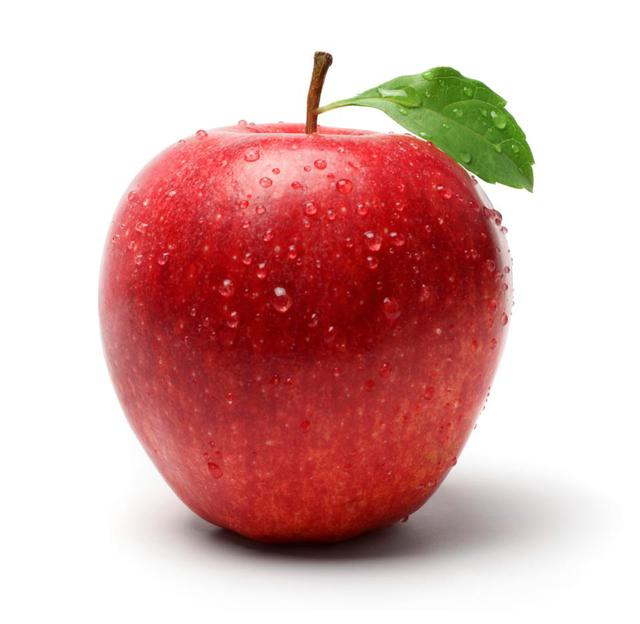
\includegraphics[width=\linewidth]{pics/domainnet/real_009_000025.jpg}
  \\(a) Real
\end{minipage}\hfill
\begin{minipage}[b]{0.27\textwidth}
  \centering
  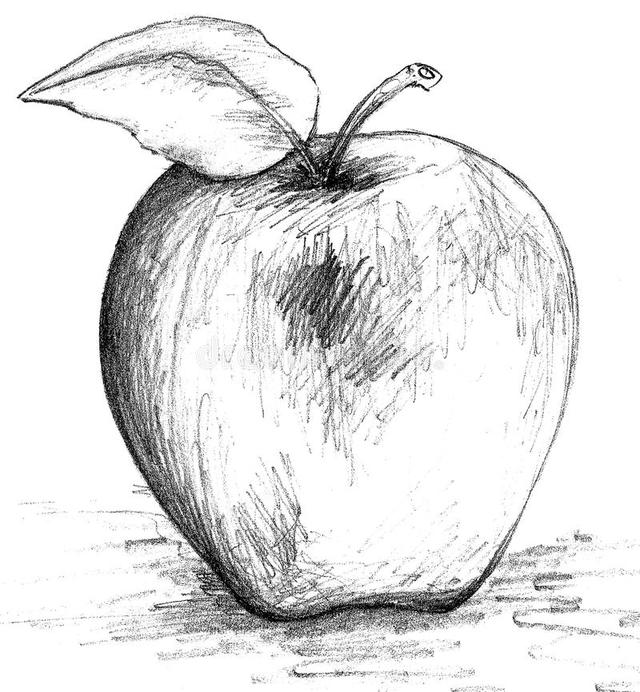
\includegraphics[width=0.8\linewidth]{pics/domainnet/sketch_009_000012.jpg}
  \\(b) Sketch
\end{minipage}\hfill
\begin{minipage}[b]{0.27\textwidth}
  \centering
  
\includegraphics[width=\linewidth]{pics/domainnet/clipart_009_000013.jpg}
  \\(c) Clipart
\end{minipage}

\vskip 1em

\begin{minipage}[b]{0.27\textwidth}
  \centering
  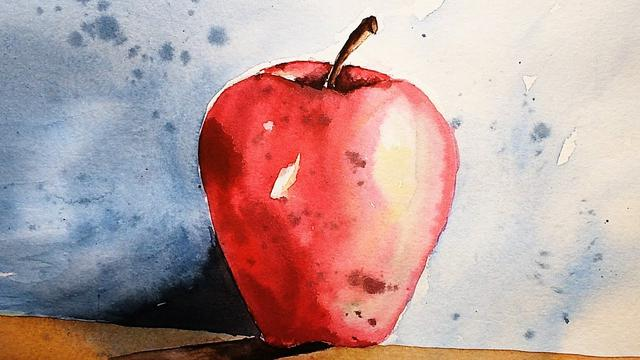
\includegraphics[width=\linewidth]{pics/domainnet/painting_009_000004.jpg}
  \\(d) Painting
\end{minipage}\hfill
\begin{minipage}[b]{0.27\textwidth}
  \centering
  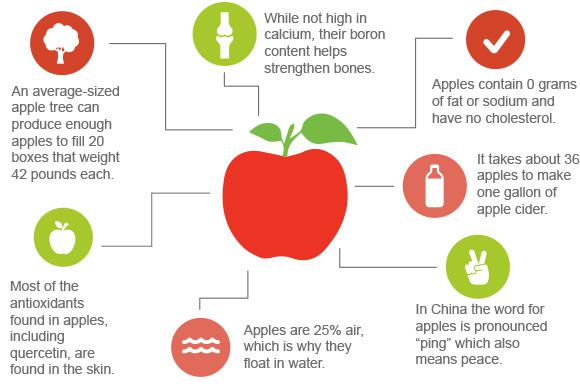
\includegraphics[width=\linewidth]{pics/domainnet/infograph_009_000020.jpg}
  \\(e) Infograph
\end{minipage}\hfill
\begin{minipage}[b]{0.3\textwidth}
  \centering
  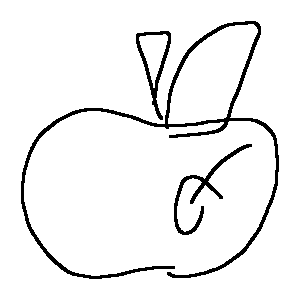
\includegraphics[width=0.7\linewidth]{pics/domainnet/quickdraw.png}
  \\(f) Quickdraw
\end{minipage}

\caption{Representative examples from the DomainNet domains: Real, Sketch, Clipart (top row); Painting, Infograph, Quickdraw (bottom row).}
\label{fig:domainnet}
\end{figure}

\subsection{Instruction tuning tasks: small-scale experiments}
\label{appendix:instruction-tuning-small}

We evaluated our CADS‐S approach on instruction fine‐tuning tasks using the GPT-2 model~\cite{Radford2019LanguageMA}. The dataset consists of two heterogeneous data sources: (i) \textbf{Alpaca-GPT4}~\cite{alpaca-gpt4}, a high-quality dataset from GPT-4-generated instructions, from which we sample \(1{,}000\) examples to simulate the rarity of premium data sources in practical scenarios; (ii) \textbf{Alpaca}~\cite{alpaca}, a larger dataset containing \(9{,}000\) examples, representing standard-quality data. The total compute budget varies within the range \([1\times10^{4},5\times10^{4}]\) sample usages. 
The selection weight \(s\) is initialized to \(0.5\cdot \bm{1}^{|D|}\). We solve the bilevel problem with AdamW for both model parameters \(\theta\) (learning rate \(1\times10^{-5}\)) and selection weights $\bm{s}$ (learning rate \(5\times10^{-2}\)). We adopt the GPT-2 backbone with maximum sequence length \(1024\) for all runs.

\paragraph{Data preprocessing.}  
Raw instruction–response samples are loaded from JSON or JSONL files and consolidated into a flat record list. A pretrained tokenizer is initialized and extended to include five special markers: a padding token, an end‐of‐sequence token, and three role‐demarcation tokens (<|system|>, <|user|>, <|assistant|>). Each record is then serialized into a single text sequence by:
\begin{enumerate}
  \item Emitting the system token, followed by the system‐level directive, and two line breaks.
  \item Emitting the user token, followed by the instruction text (and any optional input), and two line breaks.
  \item Emitting the assistant token, followed by the target response, and terminating with the end‐of‐sequence token.
\end{enumerate}
The concatenated text is first tokenized without truncation to measure its length; any example that exceeds the maximum allowed token count is discarded. The remaining examples are split into training, validation, and test subsets according to either explicitly provided sizes or a default 90/5/5 ratio.
At training time, each sequence is tokenized with truncation to the maximum length, producing token identifiers and attention masks. All token positions corresponding to the system and user segments are assigned an ignore index in the label sequence so that only assistant‐response tokens contribute to the loss. A bespoke collation routine then pads every batch to the length of its longest sequence, using the padding token for inputs, zeros for masks, and the ignore index for both prompt and padding positions in the labels. 

\subsection{Instruction tuning tasks: scaling to additional datasets}

We extended our evaluation to 13 distinct instruction‐following corpora, drawing ten thousand examples from each. These included the original AlpacaGPT4 benchmark\cite{alpaca-gpt4}, the SlimOrca set\cite{slimorca}, the Alpaca collection\cite{alpaca}, the GPTeacher suite\cite{gpteacher}, and nine multilingual variants of the Alpaca data. In total, approximately 130 000 samples were processed with the identical tokenization, formatting, filtering, and batch‐collation pipeline described above. The complete list of datasets, along with their sizes and licenses, is summarized in Table~\ref{tab:stat_data}.

\begin{table}[h]
    \centering
    \renewcommand\arraystretch{1.3}
    \setlength{\tabcolsep}{1.5mm}
    \begin{tabular}{lcr}
        \toprule
        Dataset & Size & License \\
        \midrule
        AlpacaGPT4~\citep{alpaca-gpt4}        & 52K & Apache-2.0 \\
        SlimOrca~\citep{slimorca}            & 518K & MIT        \\
        GPTeacher~\citep{gpteacher}          & 89K & MIT        \\
        Alpaca~\citep{alpaca}                & 52K & Apache-2.0 \\
        \midrule
        Alpaca-es\tablefootnote{\url{https://huggingface.co/datasets/bertin-project/alpaca-spanish}} & 52K & CC-BY-4.0        \\
        Alpaca-de\tablefootnote{\url{https://huggingface.co/datasets/mayflowergmbh/alpaca-gpt4_de}}     & 50K & Apache-2.0       \\
        Alpaca-ja\tablefootnote{\url{https://huggingface.co/datasets/fujiki/japanese_alpaca_data}}    & 52K & CC-BY-NC-SA-4.0  \\
        Alpaca-ko\tablefootnote{\url{https://huggingface.co/datasets/Bingsu/ko_alpaca_data}}         & 50K & CC-BY-NC-4.0     \\
        Alpaca-ru\tablefootnote{\url{https://huggingface.co/datasets/IlyaGusev/ru_turbo_alpaca}}      & 30K & CC-BY-4.0        \\
        Alpaca-it\tablefootnote{\url{https://huggingface.co/datasets/mchl-labs/stambecco_data_it}}    & 52K & CC-BY-NC-SA-4.0  \\
        Alpaca-fr\tablefootnote{\url{https://huggingface.co/datasets/jpacifico/French-Alpaca-dataset-Instruct-55K}} & 55K & Apache-2.0       \\
        Alpaca-zh\tablefootnote{\url{https://huggingface.co/datasets/llm-wizard/alpaca-gpt4-data-zh}}  & 49K & CC-BY-4.0        \\
        Alpaca-pt\tablefootnote{\url{https://huggingface.co/datasets/dominguesm/alpaca-data-pt-br}}   & 52K & CC-BY-NC-4.0     \\
        \bottomrule
    \end{tabular}
    \vskip 0.2in
    \caption{Summary of high‐quality instruction‐tuning datasets (top) and multilingual Alpaca variants (bottom).}
    \label{tab:stat_data}
\end{table} 
